
\documentclass[12pt,a4paper]{article}

\usepackage{fontspec}

\usepackage[BoldFont]{xeCJK}

\setCJKmainfont{DFKai-SB}                % 中文字型使用標楷體

\setmainfont{Times New Roman}          % 如果英文字型是 Times New Roman 則取消這行註解

\XeTeXlinebreaklocale "zh"             % 這兩行一定要加,中文才能自動換行

\XeTeXlinebreakskip = 0pt plus 1pt     % 這兩行一定要加,中文才能自動換行

\usepackage{geometry}

\geometry{
 a4paper,
 left=12.7mm,       %左邊界
 right=12.7mm,      %右邊界
 top=12.7mm,        %上邊界
 bottom=12.7mm,     %下邊界
 }

\usepackage{amssymb}

\usepackage{mathtools}

\usepackage{microtype}

\usepackage{enumitem}

\usepackage{dirtytalk}

\usepackage{subcaption}

\usepackage{fancyhdr}

\usepackage{graphicx}

\usepackage{indentfirst}

\usepackage{hyperref}

\usepackage{zhnumber}

\zhnumsetup{style=Traditional}

\usepackage[backend=biber]{biblatex}

\addbibresource{references.bib}

\AddEnumerateCounter{\zhdig}{\zhdig}{}

\DeclareCaptionLabelSeparator{custom}{、 }

\usepackage[justification=centering,figurename={},tablename={},labelsep=custom]{caption}

\renewcommand{\thetable}{表\zhdig{table}}

\renewcommand{\thefigure}{圖\zhdig{figure}}

\renewcommand{\tableautorefname}{}

\pagestyle{fancy}

\fancyhead{} % 清除所有頁首設定

\fancyfoot{}

\renewcommand{\headrulewidth}{0pt}

\renewcommand{\footrulewidth}{0pt}

\setlength{\headwidth}{\textwidth}

\lfoot{表 C802}

\rfoot{共~~\pageref{LastPage}~~頁~~第{~~\thepage~~}頁}

\begin{document}

\setlength{\parindent}{2em}

\noindent{\bf \large  二、 研究計畫內容:}

\begin{enumerate}[label={(\zhdig*)}, leftmargin=2\parindent, listparindent=\parindent]

\item 摘要

    隨著微服務 (Microservices) 和雲原生技術 (Cloud-native) 的普及,現代
    應用系統高度依賴 高併發 API 服務,應用於金融交易、電商促銷、影音
    串流、物聯網等場景,並對 低延遲、高可用性與動態擴展 提出了嚴格要求。
    例如:

    金融交易 API 需要毫秒級延遲來確保最佳買賣時機,對資源調度與計
    算負載有極高要求。交易峰值可能在短短幾秒內增加數十倍,若 API 擴展
    反應過慢,可能導致交易失敗或市場損失。[3]

    大型電商平台促銷活動期間(如雙 11 促銷活動),大量用戶同時請求
    API 進行商品查詢、購物車更新、訂單提交,瞬間請求量可達數百萬 QPS
    (Queries Per Second)。傳統的 API 擴展方式無法即時應對流量暴增,可
    能導致購物車服務崩潰、支付 API 超時,影響用戶體驗與企業營收。[4]

    社群媒體與影音串流(如 TikTok、YouTube、Instagram)用戶大量發送
    請求以獲取動態、影片內容,並伴隨 AI 推薦計算(如 TikTok For You Feed)。
    服務需要即時擴展,確保推播內容的低延遲傳遞,同時兼顧後端機器學習推
    理任務的負載平衡。[5]

    物聯網 (IoT) 平台(如智慧城市、工業 4.0)則是有大量 IoT 設備持續
    發送感測數據至雲端 API 進行分析、存儲,且流量具有明顯的時段性波動
    (如白天比晚上流量高)。若 API 無法適應 IoT 端的流量模式,可能導致
    數據擷取延遲或設備無法連接雲端,影響關鍵應用(如智慧交通信號調度)。
    [6]

    然而,現有的 Kubernetes VPA (Vertical Pod Autoscaler) 和 CA (Cluster
    Autoscaler) 在高併發環境下仍存在 資源調度延遲、負載預測不準確與異構
    計算資源適配困難 等挑戰。
    目前的 VPA 僅依賴 CPU/Memory 負載 來觸發擴展,無法預測即將到
    來的請求流量,導致擴展決策延遲,影響 API 響應時間與穩定性。因此,
    本研究旨在透過深度學習與強化學習技術,提升 API 調度與擴展策略,開
    發一套 負載預測、智能調度與 SLA 自適應擴展系統,以降低 API 響應時
    間、提高資源利用率,並確保高併發環境下的服務穩定性。

\item 研究動機與研究問題(600字)\label{研究動機}

\begin{enumerate}[label={(\arabic*)}, leftmargin=\parindent, listparindent=\parindent]

\item\textbf{虛擬化技術(Virtualization)[8]}

    虛擬化技術最早可追溯到 1960 年代,最初應用於大型主機(Mainframe)
    系統,用於同時支援多個使用者與處理多道程序。隨著硬體計算資源不斷提
    升,虛擬化開始普及到商用伺服器領域,並逐漸成為許多企業基礎建設的核
    心要素。所謂「虛擬化」,簡單來說就是將實體硬體資源透過軟體抽象化,
    從而建立出多個「虛擬機(Virtual Machine, VM)」。這些虛擬機由「虛擬機
    管理程式(Hypervisor)」進行控制與協調,每個虛擬機都可以擁有自己的作
    業系統、應用程式與設定檔,並且彼此間互不干擾。

    Hypervisor 大致可分為兩類:Type 1(裸機式)與 Type 2(宿主機式)。
    Type 1 Hypervisor 可以直接安裝在硬體之上,如 VMware ESXi、Microsoft
    Hyper-V、Xen 等,是大多數企業級虛擬化解決方案的基礎;Type 2
    Hypervisor 則運行在現有作業系統上,如 VMware Workstation、Oracle VM
    VirtualBox 等,常用於開發者在本地測試或個人環境中快速建立虛擬機。

    虛擬化技術帶來的第一個好處是硬體資源的充分利用。在未採用虛擬化
    的情況下,企業往往需要購買多臺實體伺服器來執行不同的應用程式,容易
    造成硬體閒置或資源浪費。透過虛擬化,單一硬體可被切分成多個虛擬機,
    讓同一臺伺服器能同時執行多個作業系統與服務,大幅提升資源使用率。第
    二個好處是環境隔離:每個 VM 都有獨立的 OS 與應用程式堆疊(Stack),
    彼此之間不會互相干擾或資源競奪,可有效避免衝突問題。第三個好處則是
    彈性與可移植性:透過虛擬化技術,可以輕易地將整個 VM(包括 OS、應
    用程式與設定)從一臺實體機器移轉到另一臺,達到熱遷移(Live Migration)
    與彈性升級的目標,這對於維運管理與災難復原(Disaster Recovery)都極
    具幫助。

    然而,虛擬化技術也並非完美無缺。由於每個虛擬機都需要整套 OS 核
    心以及系統檔案,硬體資源的佔用量相對較高;當企業需要大規模水平擴充
    (Horizontal Scaling)時,必須同時建置或複製許多 VM,管理與維運的複
    雜度也會顯著增加。儘管如此,虛擬化依然是大型資料中心與企業私有雲建
    設的一大支柱,因為它能在單一硬體上容納多個異質性環境(不同 OS、不
    同應用程式),大幅提升系統部署與維運的效率。

    在當前混合雲與多雲的時代,虛擬化依然扮演重要角色。即使後來興起
    的容器化技術(Containerization)在許多應用場景中更加輕量與快速,但許
    多核心服務或需要完整 OS 隔離的應用,仍然持續仰賴虛擬化來提供安全
    與穩定的基礎執行環境。這意味著虛擬化與容器化並非絕對排斥或相互取
    代的關係,反而可以在多層架構中協同並行:有些組織會在虛擬機內部再運
    行容器,或者同時維持 VM 與容器協作,以達到最有效的資源配置。
\item\textbf{
容器化技術(Containerization)[9]
}

容器化技術興起的背景,與虛擬化技術的侷限性不無關係。虛擬化雖然
解決了一機多用與環境隔離等問題,但因為每個虛擬機都需要整套作業系
統核心,使得其在資源佔用、啟動速度與可移植性方面並非最理想。隨著互
聯網服務對資源彈性與佈署速度的要求越來越高,容器化技術作為「更輕
量、更靈活」的解決方案逐漸嶄露頭角。其中,最具代表性的就是 Docker,
它在 2013 年正式開源,並迅速引發業界熱烈關注。

「容器化」的核心概念在於:每個容器(Container)只在應用層進行隔
離,而不需要為每個容器重複攜帶一整個作業系統核心。容器與宿主機
(Host)共享同一個 OS Kernel,但彼此之間仍透過 Linux NameSpaces、
Control Groups(cgroups)等機制來保持獨立的檔案系統、網路配置與系統
資源限制。因此,容器可以被視為「進程級(Process-level)」的虛擬化:它
只將應用程式與必要的函式庫、設定檔打包進「映像檔(Image)」裡,而非
把整個 OS 都複製一份。這帶來幾個重要好處:
\begin{itemize}[leftmargin=\parindent, listparindent=\parindent]

\item\textbf{輕量化:}由於容器不需額外攜帶整套 OS,映像檔體積通常遠小於虛擬
機磁碟映像,容器的啟動速度也更加迅速,可以在數秒甚至更短時間內完成
部署。

\item\textbf{高可移植性:}容器映像檔在任何安裝了容器執行環境(如 Docker Engine、
containerd)的系統上都可以運行,無論該系統是公有雲、私有雲或是本地
伺服器,極大地降低了「環境差異」帶來的問題。
一致性:開發人員可以在開發階段就打包好所有依賴函式,確保在測試與生
產環境中執行的應用具備相同的軟體堆疊,避免了「在我機器上可以跑」的
常見爭議。

\item\textbf{快速伸縮}:由於容器能夠快速啟動與關閉,當流量快速上升時,可以透
過增加容器實例來應付瞬時負載;相對地,當流量下降時,也能及時縮減容
器實例以節省資源成本。
\end{itemize}

Docker 是推動容器化技術普及的主要力量,其易用的命令列工具與
Dockerfile 定義方式,讓開發者能夠輕鬆撰寫出構建映像檔的流程,並在本
地端進行快速測試。此後,圍繞 Docker 所延伸出的生態系統與技術標準也
相當豐富,包括 Registry(映像檔儲存庫)、Compose(多容器編排)、Swarm
(容器集群管理)等。即便後來 Kubernetes 在容器編排領域成為主流,
Docker 在容器映像打包與基本執行環境上的地位仍相當關鍵。

不過,容器化並不等同於「一勞永逸」。當應用服務架構逐漸演化成包含
數十、數百甚至數千個容器時,如何協調這些容器的部署、資源分配、健康
檢查、日誌管理,以及版本更新,就成為更巨大的挑戰。這也是為什麼
Docker 開源之後,快速催生了各類容器編排工具(如 Docker Swarm、
Apache Mesos 與 Kubernetes),其中以 Google 開發並開源的 Kubernetes
最終成為「事實標準」。

\item\textbf{
Kubernetes[9]
}

Kubernetes,通常縮寫為 K8s,由 Google 於 2014 年以開源方式釋出,
現已成為容器編排(Orchestration)領域的事實標準。它的核心目標是自動
化部署、管理、監控並擴展容器化應用程式,讓開發與運維團隊不再需要為
大量容器的協調工作煩惱。Kubernetes 的誕生源自 Google 內部多年的大
規模容器運行經驗,畢竟 Google 自家也在龐大的分散式系統中廣泛運用
容器技術,而 Kubernetes 可以被視為他們在 Borg 與 Omega 等內部系統
基礎上抽象、改良而來的精華。

在 Kubernetes 中,最基本的運行單元稱為 Pod。一個 Pod 可以包含一
個或多個彼此緊密相關的容器,它們共享網路命名空間與儲存空間,但在邏
輯上被視為一個整體,通常用於部署同一個微服務或同一個組件的多個容
器。多個 Pod 組合起來,再透過各種 Kubernetes 物件如 Service、
Deployment、ReplicaSet 等,構成整個應用系統。以下是 Kubernetes 的幾
項核心功能與特點:

\begin{itemize}[leftmargin=\parindent, listparindent=\parindent]
\item\textbf{
自動伸縮(Autoscaling):}Kubernetes 提供多種伸縮機制,如 Horizontal
Pod Autoscaler,能監控 Pod 的 CPU 或記憶體使用率,或其他自訂指標,
根據需求自動增減 Pod 的數量。當流量驟增時,系統可以快速啟動更多容
器以應對;當流量下降時,又能縮減容器以節省成本。

    \item\textbf{
滾動更新與回滾:}在傳統運維模式下,更新應用程式常需要停機維護;
但在 Kubernetes 中,Deployment 能實現「滾動更新」,讓新版本的容器與
舊版本容器同時存在,逐步替換,期間使用者不會感受到中斷。如果更新後
出現嚴重問題,也能透過回滾功能(Rollback)立即恢復到上一個穩定版本,
將風險降到最低。

    \item\textbf{
故障自動修復:}Kubernetes 會持續監控容器與 Node 的狀態,一旦發現
某個 Pod 出現問題或某個 Node 不可用,就會重新在其他可用 Node 上
啟動新的 Pod。這種自動修復機制能確保整體服務不會因個別故障而停擺。

    \item\textbf{
豐富的生態系統:}Kubernetes 本身只是核心框架,社群提供了大量的附
加元件(Add-ons)、套件(Helm Chart)、網路插件(CNI 插件),甚至雲廠
商也為 Kubernetes 提供了托管服務(如 GKE、EKS、AKS),讓使用者更
容易管理叢集並整合雲平台資源。

\end{itemize}

由於 Kubernetes 通過宣告式(Declarative)的操作方式,使用者只需描
述「期望狀態」(Desired State),系統就會不斷調整並確保實際狀態符合這
個期望狀態,減少了許多繁瑣的人工作業與配置錯誤。這種架構也非常契合
DevOps 與 GitOps 的流程,能與持續整合/持續交付(CI/CD)工具相結合,
以達到自動化部署應用的目標。

\item\textbf{微服務(Microservices)[10]}

微服務(Microservices)是一種軟體架構風格,旨在將龐大而複雜的應
用程式拆分成若干小規模、可獨立部署與維護的服務模組。每個服務都聚焦
於特定的業務功能,如使用者管理、訂單處理、付款系統等,彼此之間透過
輕量級通訊協定(大多是 HTTP 或 gRPC)互相協作。相較於傳統的單體
式(Monolithic)應用,微服務架構更能應對現代企業對快速迭代、彈性擴
充與分散式團隊合作的需求。

在單體應用中,所有功能模組都綁定在同一個可執行檔或程式集中,一
旦有任一模組需要更新,就必須重新部署整個應用,且可能引發相依性衝突
或造成服務中斷。微服務則透過將功能拆分到各個獨立服務的方式,賦予了
開發團隊更高的自主性:每個微服務可選擇最適合自身需求的程式語言、資
料庫與技術棧(Tech Stack),而不需要受到整體專案的限制。這種模式使「單
一職責原則(Single Responsibility Principle)」落實到整個系統設計中,每個
微服務都只專注於自家功能。

除了開發層面的靈活度,微服務也帶來了在部署與維運上的優勢。透過
容器化技術,每個微服務都能打包成獨立的容器映像檔,並在任何支援容器
的環境中運行。再結合 Kubernetes 或其他容器編排工具,就能為每個微服
務獨立設定伸縮策略。例如,若「訂單處理」模組在購物季節流量飆升,運
維人員或系統可自動擴增該微服務的容器副本,而不需要同步擴增其他服
務;反之,當流量回落,則可縮減至一般量級,避免資源浪費。這種彈性伸
縮的能力對於現代網路服務尤為關鍵。

然而,微服務的導入也伴隨著複雜度的提升。系統從單一執行檔拆分成
數十甚至數百個微服務後,如何確保跨服務的資料一致性?如何進行服務
發現(Service Discovery)與健康檢查?如何管理版本更新與相依性?以及,
如何在分散的日誌與監控訊息中追蹤整體系統健康狀態?這些議題都是微
服務落地時必須面對的挑戰。為了解決此問題,企業往往需要導入更完整的
DevOps 工具鏈、API Gateway、服務網格(Service Mesh)等基礎設施,並
在設計初期就考慮到可觀察性(Observability)與故障容忍(Fault Tolerance)。

儘管如此,微服務帶來的高彈性與可維護性,仍使其成為大多數互聯網巨頭
與新創公司首選的架構模式。微服務可讓不同的開發團隊各自負責特定功
能領域,以更快的速度開發與部署新功能,也便於持續整合/持續交付
(CI/CD)的落實。對於迅速變動的市場需求與多端服務(Web、App、IoT
裝置)的支援,微服務可輕鬆因應,以小步快跑的方式持續優化。

\item\textbf{雲原生技術(Cloud-native)}

「雲原生(Cloud-native)」是一個在近幾年被廣泛談及的概念,但它並
非指單一技術或架構,而是涵蓋一系列以雲端為主要運行環境與思維基礎
的軟體開發與部署模式。雲原生的核心精神,可以用 CNCF(Cloud Native
Computing Foundation)的定義來概括,即利用容器、微服務、動態編排與
API 驅動的基礎設施,來構建可彈性伸縮且易於管理的分散式系統。

在雲原生理念下,應用程式的開發與運行從一開始就要考慮到雲端環境
的特性,包括自動伸縮、分散式部署、服務網路以及故障快速恢復等。這些
特性直接影響了系統設計與開發流程:傳統的單體式應用往往難以快速擴
充或橫向拆分,而雲原生更鼓勵應用被拆解成微服務,並運行在容器之中,
再透過 Kubernetes 等編排工具集中管理。如此一來,系統就能根據負載的
變動自動增加或減少容器實例,不需要過多的人為干預。

雲原生還強調敏捷開發與 DevOps 文化的深度融合。在過去,開發團隊
與運維團隊之間常常存在明顯的分工界限:開發負責寫程式,運維負責部署
與管理伺服器。然而,在雲原生的世界裡,應用的版本更新往往是透過
CI/CD(持續整合/持續交付)管線自動化完成,應用的一切依賴(包括程式
語言版本、函式庫、系統參數設定)都在容器映像檔中定義好,使得同一套
環境能從測試階段無縫遷移到正式生產環境。同時,宣告式(Declarative)
的運維方式也大幅降低了人工作業失誤的風險,使整個軟體開發生命週期
更加流暢。

另一個雲原生的重要面向是可觀察性(Observability)。在傳統單體應用
時代,系統多半由一個或少數大型進程組成,出現問題時還能相對容易地進
行除錯或分析;但在雲原生架構下,系統通常由眾多微服務協同運作,每個
微服務又可能進行水平擴充,產生大量容器。若沒有良好的日誌、指標
(Metrics)與分佈式追蹤(Tracing)機制,開發與維運人員會難以掌握系統
狀態與故障根源。為此,雲原生體系常搭配 Prometheus、Grafana、Jaeger 等
工具,以及微服務之上的 服務網格(Service Mesh)方案(如 Istio、Linkerd),
協助解決通訊與觀察性問題。

另外,多雲(Multi-cloud)與混合雲(Hybrid Cloud)也是雲原生技術
的重要延伸趨勢。許多企業不滿足於只使用單一公有雲供應商,而是會在公
有雲、私有雲與本地機房間彈性部署應用。這就需要應用擁有高度的可移植
性與跨平台支援,容器與 Kubernetes 也在這裡發揮關鍵作用:只要可以在
各平台安裝 Kubernetes,就能擁有統一的部署與管理介面,不受底層環境
差異影響。

\item\textbf{現有 Kubernetes 擴展機制的挑戰}

目前,許多企業採用 Kubernetes(K8s) 來管理雲端資源,並透過 VPA
(Vertical Pod Autoscaler) 和 CA (Cluster Autoscaler) 來應對流量變化。然
而,這些現有擴展機制在高併發 API 服務場景下仍存在以下關鍵問題:
\begin{itemize}[leftmargin=\parindent, listparindent=\parindent]
    \item\textbf{資源調度延遲:}

Kubernetes VPA 依賴 CPU / Memory 閾值監測 來觸發 Pod 擴展,然而
這種方式屬於被動式反應:
VPA 需要等到 CPU / Memory 負載超過閾值後才開始擴展,這意味著
系統已經開始過載才會進行調整,並且 VPA 整體擴展過程也會具有一定延遲,從而導致 API 服務短期內請求失
敗率上升。

    \item \textbf{
負載預測不準確
}

VPA 無法提前預測 API 流量模式,而是單純依賴當下的 CPU /
Memory 使用率,這在應對突發性高併發流量時顯得效率低下:
無法預測即將到來的高流量:例如電商促銷開始前的 API 請求量通常
會呈指數級增長,但 VPA 在負載真正升高前不會觸發擴展,導致初期請求
可能被拒絕。
無法學習歷史數據:VPA 不會根據歷史流量模式來調整策略,無法針對
每天固定時段的高峰流量(如午餐時段、晚間流量高峰)做出提前擴展的決
策。[7]

    \end{itemize}
    \item \textbf{研究動機與目標}

鑑於上述挑戰,本研究的動機在於透過深度學習與強化學習技術,解決
Kubernetes 在高併發 API 服務中的智能調度與自適應擴展問題。

本研究的目標是:
\begin{itemize}[leftmargin=\parindent, listparindent=\parindent]

    \item 設計基於深度學習(RNN/CNN)的負載預測模型,提前預測 API 流量
變化,減少 VPA 反應延遲。
開發基於強化學習(RL)的 Kubernetes Scheduler,根據 API 請求負載與
異構計算資源的特性,最佳化 Pod 調度策略,提高 GPU/NPU 運算效率。

    \item 建立 SLA 驅動的自適應 Cluster Autoscaler(SAA),根據 API 響應時
間與請求成功率,動態調整 CA 擴展策略,確保高併發服務的穩定性。
透過這套智能調度與擴展系統,本研究將能夠降低 API 響應時間、提升資
源利用率、減少高流量衝擊下的請求失敗率,進而提高 API 服務的穩定性
與效能。
\end{itemize}

\end{enumerate}
\item 文獻回顧與探討(600字)

容器調度(Container Scheduling)是雲計算和邊緣計算領域的重要研究
課題,其目標是在動態環境中有效管理資源,確保負載均衡、降低能源消耗
並提升應用效能。現有的研究方法可分為\textbf{數學建模(Mathematical
Modeling)、啟發式演算法(Heuristic Algorithms)、元啟發式演算法(MetaHeuristic Algorithms)、機器學習(Machine Learning)}等不同類別,本文
將基於近期的研究成果進行綜合探討。
\begin{enumerate}[label={(\arabic*)}, leftmargin=\parindent, listparindent=\parindent]

    \item \textbf{
啟發式演算法:區域性感知與多目標調度}

啟發式演算法通常透過經驗法則和啟發資訊進行資源分配,較適用於即
時調度需求,但易受局部最優解影響。
\begin{itemize}[leftmargin=\parindent, listparindent=\parindent]
    \item \textbf{
[11] 區域性感知(Locality-Aware)調度}

Diego 等人提出了一種區域性感知(Locality-Aware)的調度機制,透過
統計方法將負載均衡(Load Balancing)與應用效能(Application Performance)
統一為一個優化問題,以降低 I/O 和網路流量瓶頸。該方法適用於資料密
集型應用,並在 CloudFoundry 平台上驗證了其效能優勢。
\item \textbf{
[12] Multiopt:多目標最佳化調度
}

Multiopt 是一種基於多目標最佳化(Multi-Objective Optimization)的調
度方法,綜合考量 CPU 使用率、記憶體使用率、網路傳輸時間、容器與節
點的關聯性、容器聚類等五個因素,透過計分函數(Scoring Function) 選
擇最佳節點來部署容器,進一步提高系統的吞吐量(TPS)並降低平均響應
時間。

    \end{itemize}
    \item \textbf{
元啟發式演算法:螞蟻、粒子群與混合演算法
}

元啟發式演算法(Meta-Heuristic Algorithms)利用啟發資訊進行全域搜
尋,適用於複雜調度問題,但計算開銷較高。
\begin{itemize}[leftmargin=\parindent, listparindent=\parindent]
    \item \textbf{
[13] MOO-ACA,GA-MOCA:基於螞蟻演算法(ACO)的容器調度}

MOO-ACA 透過螞蟻演算法(Ant Colony Algorithm, ACO)來考量網路
傳輸開銷、負載均衡與服務可靠性,運用費洛蒙更新機制提升全域最適性,
使得容器調度更符合雲端環境的變動需求。

    \item \textbf{


[14] EECS 與 APSO:基於粒子群最佳化的能效調度
}

EECS 採用加速粒子群最佳化(APSO)演算法,透過權重加總法
(Weighted-Sum Method)來同時考量計算時間與能源消耗,並透過**規則
式策略(Rule-Based Strategy)**確保容器分配的合理性,進而降低雲端數
據中心的總能源消耗。

\end{itemize}
    \item \textbf{
容器虛擬化與軟體定義數據中心(SDDC)調度策略
}

容器虛擬化技術(Container-Based Virtualization)為雲端與邊緣環境提供輕
量級虛擬化能力,並透過動態資源分配提升系統效率。
\begin{itemize}[leftmargin=\parindent, listparindent=\parindent]
    \item \textbf{
[15] 基於容器的虛擬化調度模型
    }

該研究提出了一種基於容器虛擬化的節能型工作流調度方法,透過雙向
鏈表訪問機制(Doubly Linked List-Based Access)與哈希調度(Hash-Based
Scheduling)來動態管理資源,並減少 VM 遷移開銷。該方法可在軟體定義
數據中心(SDDCs) 環境下提升能效與系統穩定性。

    \end{itemize}
    \item \textbf{
基於多準則決策分析(MCDA)的 Kubernetes 容器調度
}

多準則決策分析(MCDA)方法適用於多維度資源調度問題,可透過權
重分析與演算法結合提升決策準確性。
\begin{itemize}[leftmargin=\parindent, listparindent=\parindent]
    \item \textbf{
[16] KCSS:基於 MCDA 的 Kubernetes 容器調度策略
    }

KCSS 透過 TOPSIS 演算法,考量 CPU、記憶體、磁碟使用率、功耗、
容器數量、影像傳輸時間等六個因素,以排程完成時間(Makespan)與能源
效率為主要目標來優化 Kubernetes 調度決策。

    \end{itemize}
    \item \textbf{
當前最先進的容器調度技術總結與未來方向
}
    \begin{itemize}[leftmargin=\parindent, listparindent=\parindent]
        \item\textbf{
[17] 容器調度技術的全面調查
}

該研究將當前最先進的容器調度技術歸納為數學建模、啟發式、元啟發
式、機器學習四大類,並針對資源利用率、負載均衡、可擴展性、能效等關
鍵效能指標進行分析,指出未來研究方向應包括:AI 驅動的智慧調度(如
強化學習 Reinforcement Learning)、邊緣計算環境的適應性、跨雲與混合雲
調度策略

        \end{itemize}
\end{enumerate}
\item 研究方法及步驟
\begin{enumerate}[label={(\arabic*)}, leftmargin=\parindent, listparindent=\parindent]

\item \textbf{
系統架構總覽
}

本研究旨在解決 Kubernetes 在高併發 API 服務中的調度與自適應擴展問題,其系統架構由三大核心模組組成:負載預測 (Load Prediction)、智能調度 (Intelligent Scheduling) 及自適應擴展 (Adaptive Scaling)。這些模組彼此協作,透過 深度學習 (Deep Learning, DL) 與強化學習 (Reinforcement Learning, RL),提升 API 調度的準確性、Pod 佈署效率及資源擴展的靈活性,確保高併發場景下的穩定性與效能。

整體架構基於 Kubernetes (K8s) 平台,並整合 自訂 Kubernetes Scheduler [19]來實現更精細化的排程管理。不同於 Kubernetes 內建的 VPA (Vertical Pod Autoscaler) 和 CA (Cluster Autoscaler) 主要依賴 CPU/Memory 使用率來決定資源調度[18],本研究的系統透過 RNN (Recurrent Neural Network) 負載預測模型、DQN (Deep Q-Network) 排程器及 SLA 驅動的自適應擴展策略,提供更智能的決策機制,以 降低 API 響應時間、提高資源利用率,並減少因擴展延遲而導致的服務中斷。
\begin{enumerate}[label={(\zhdig*)}, leftmargin=\parindent, listparindent=\parindent]
\item \textbf{
系統架構組成}

\begin{itemize}[leftmargin=\parindent, listparindent=\parindent]
\\本系統架構主要包含三大核心模組,各自負責不同層級的優化:

\item \textbf{負載預測模組 (Load Prediction Module):}使用深度學習(RNN/CNN)來預測未來的 API 負載,並提前規劃資源需求,減少 Kubernetes VPA 或 CA 擴展延遲。
\item \textbf{智能調度模組 (Intelligent Scheduling Module):}透過基因演算法(GA),最佳化 Kubernetes 調度器 (Scheduler),將 Pod 分配至最佳節點,提高資源利用率並降低 API 響應延遲。
\item \textbf{自適應擴展模組 (Adaptive Scaling Module):}根據 SLA 監測 API 響應時間與請求成功率,自適應調整 Cluster Autoscaler (CA) 擴展策略,以確保高併發 API 服務的穩定性與效能。

這三大模組彼此協作,確保 API 服務能夠在高併發環境下即時預測負載、智能調度資源、動態擴展集群,提升整體效能。

\end{itemize}
    \item \textbf{
系統運作流程}

當 API 請求進入 Kubernetes 叢集時,系統將根據 API 負載變化與資源狀況,進行 動態預測、智能調度與自適應擴展,具體流程如下:
\begin{enumerate}[label={(\arabic*)}, leftmargin=\parindent, listparindent=\parindent]

    \item\textbf{
負載監測與預測}
\begin{itemize}[leftmargin=\parindent, listparindent=\parindent]

    \item 透過 RNN/CNN 模型 預測 API 服務的短期與長期流量趨勢,產生負載預測結果。
    \item 依照預測結果決定是否調用 VPA/CA 擴展模組,調整資源擴展策略,確保擴展決策更符合流量模式。
\end{itemize}
    \item\textbf{
智能調度與 Pod 部署}
\begin{itemize}[leftmargin=\parindent, listparindent=\parindent]
    \item 當有新的 API 請求或擴展需求時,智能調度模組會透過 GA 演算法,產生最佳的部署 Pod 計畫並回傳給集群使用。
\end{itemize}
\item\textbf{SLA 驅動的自適應擴展}
\begin{itemize}[leftmargin=\parindent, listparindent=\parindent]
    \item 監測 API 響應時間、請求成功率與系統資源使用狀況,判斷是否需要擴展或釋放資源。
    \item 若請求成功率下降,則透過 SLA 驅動的 CA 擴展策略 來動態調整 Kubernetes Cluster 的節點數量,確保服務穩定性。
\end{itemize}


\end{enumerate}

\end{enumerate}
    \item \textbf{
系統架構圖}

\begin{figure} [htbp]

\centering

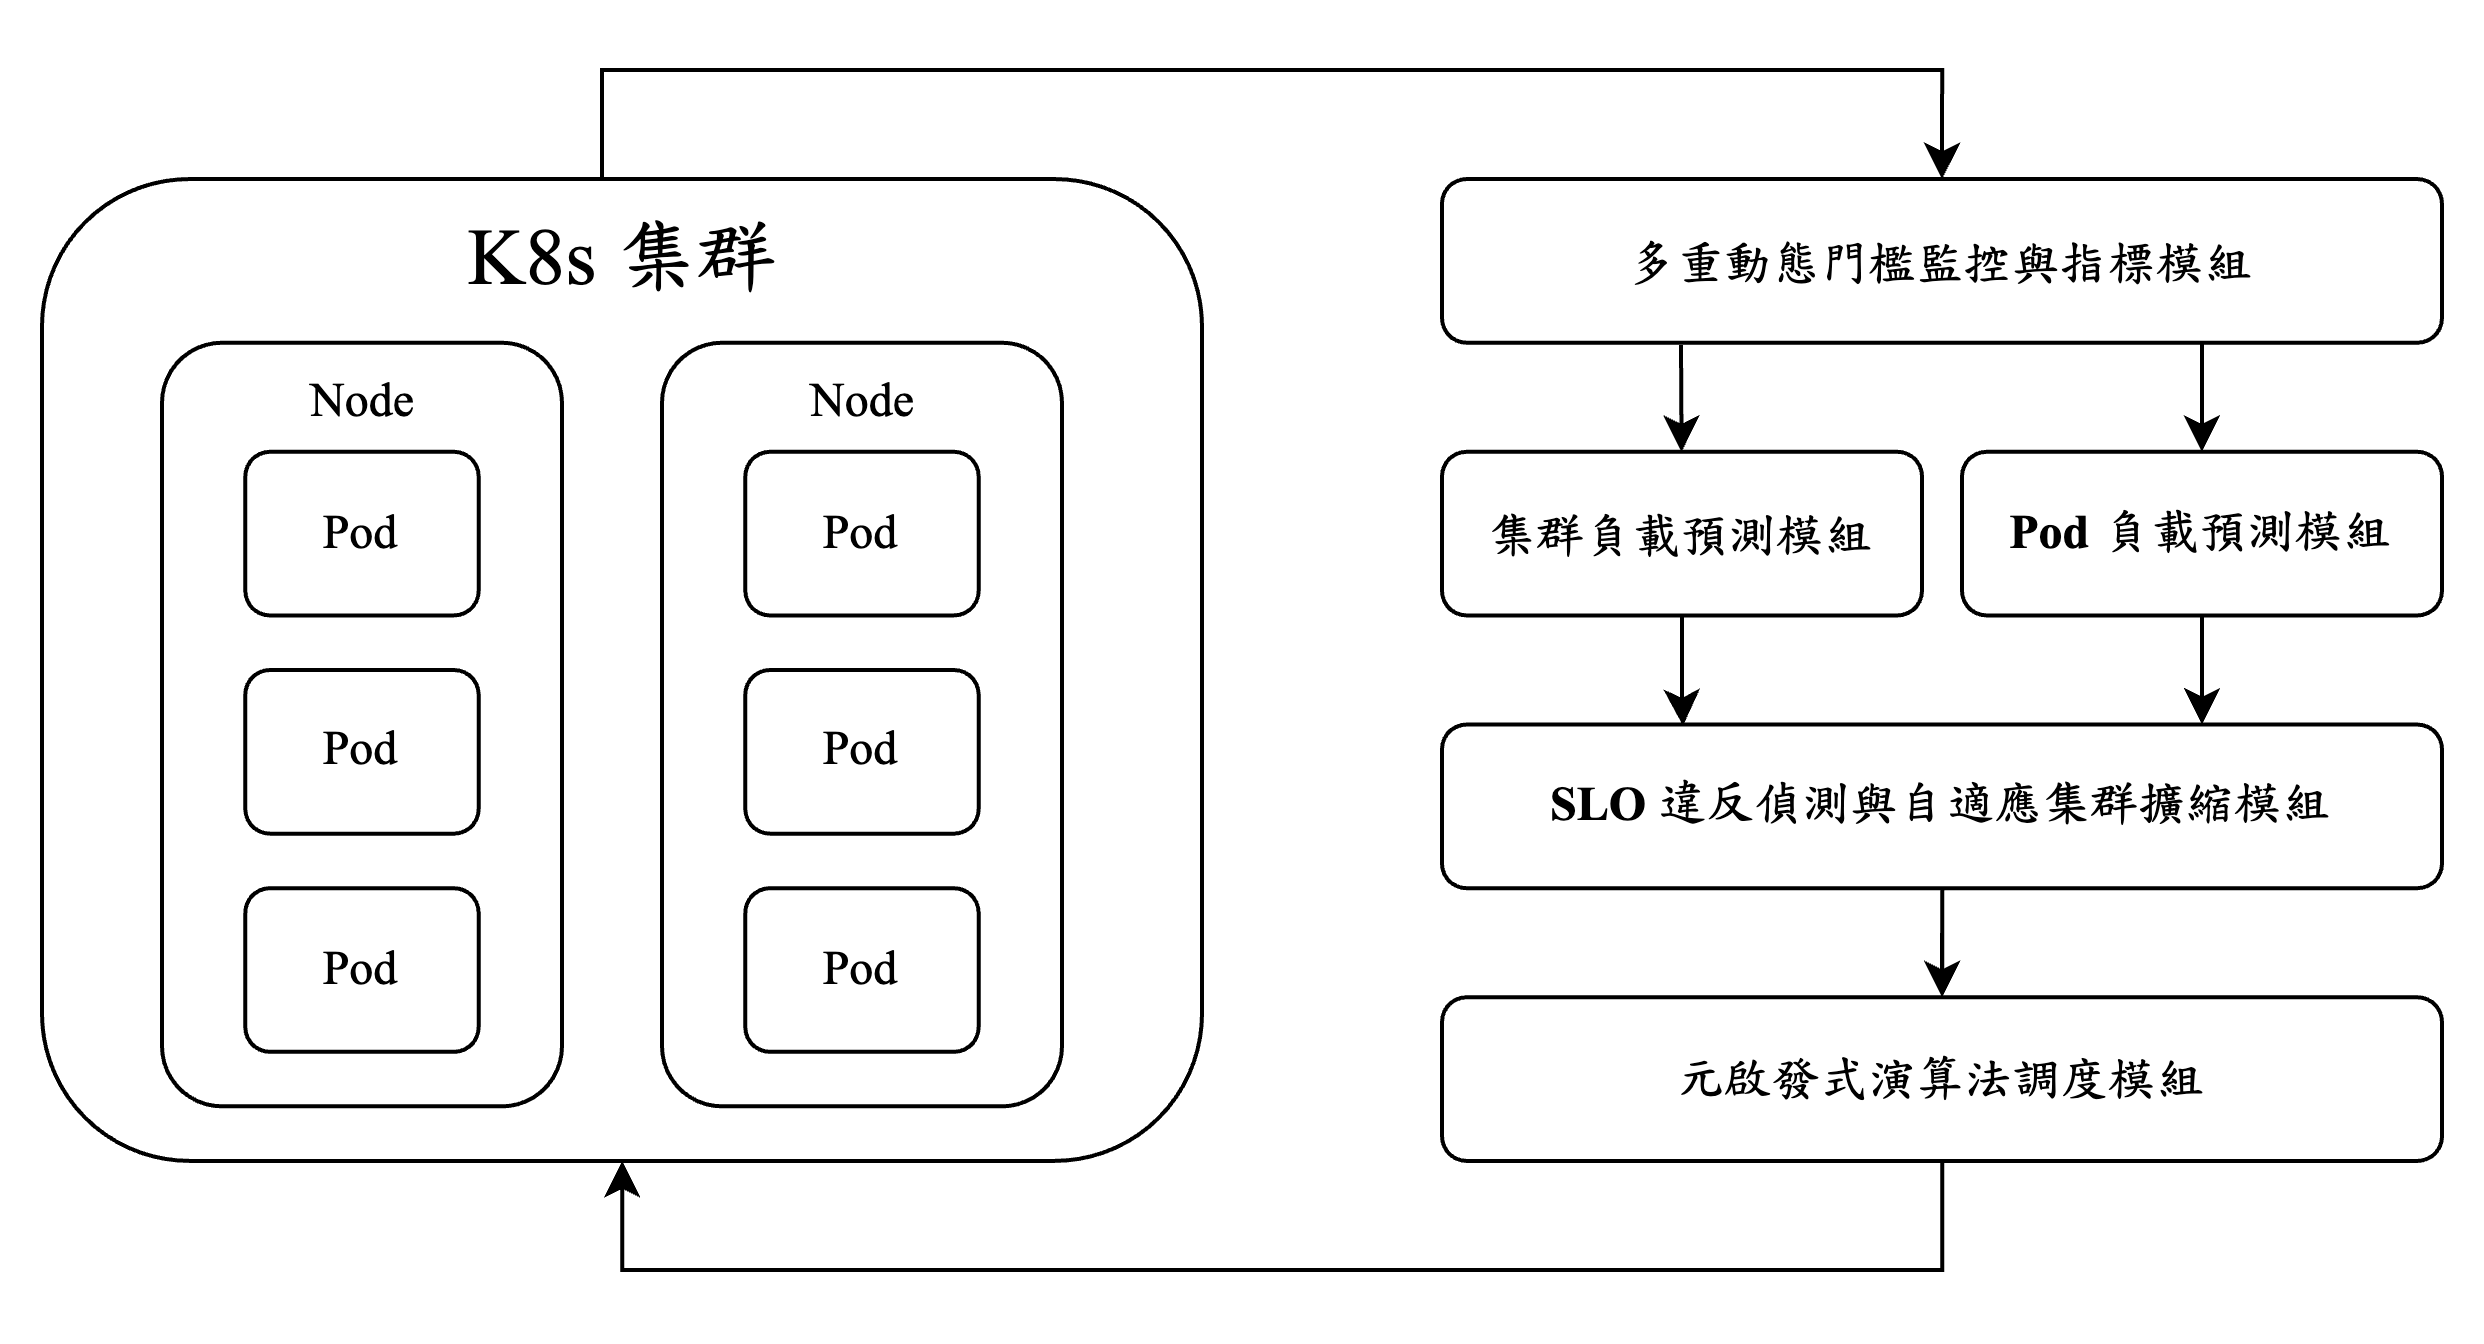
\includegraphics[width=0.9\textwidth]{fig/model.png}

\caption{架構圖}

\end{figure}\newpage

\item \textbf{
模組詳細說明}
\begin{enumerate}[label={(\zhdig*)}, leftmargin=\parindent, listparindent=\parindent]

    \item \textbf{
調度器(Scheduler)}

調度器負責根據 Cluster 內的即時資源狀況與負載預測結果,決定 Pod 部署位置。當新的 API 服務請求進入時,調度器會選擇最適合的節點來部署 Pod,確保 資源使用最佳化與負載均衡。

    \item \textbf{
服務壓力預測器(Service Load Predictor)
)}

該模組負責監測 單一 API 服務的負載變化,透過機器學習模型預測 1 到 5 分鐘內的流量趨勢,幫助 VPA 提前規劃擴展決策,減少擴展延遲問題。

\item \textbf{集群壓力預測器(Cluster Load Predictor)}

此模組負責預測整體 Kubernetes Cluster 的負載趨勢,透過學習歷史資源使用數據,分析未來 5 到 15 分鐘 的節點資源需求,並提供 Cluster Autoscaler(CA) 參考,以提升 Kubernetes 節點擴展的準確性。

 \item \textbf{VPA(Vertical Pod Autoscaler)}

當 Pod 內部資源(如 CPU 或 Memory)使用率較高時,VPA 會根據即時負載情況 自動調整 Pod 內的資源配額,避免因為資源不足而導致 Pod 效能下降或請求失敗,減少不必要的水平擴展。
\item \textbf{
集群擴展器(Cluster Autoscaler)
}

該模組根據 集群壓力預測結果,動態調整 Kubernetes Cluster 節點的數量,確保系統擁有足夠的計算資源應對 API 請求負載,避免因資源不足而導致 API 響應時間增加或請求丟失。

\end{enumerate}
\end{enumerate}
\item 預期結果

\item 需要指導教授指導內容

\item 參考文獻


\end{enumerate}


\label{LastPage}


\end{document}

